%----------------------------------------------------------------------------------------
%	PACKAGES AND OTHER DOCUMENT CONFIGURATIONS
%----------------------------------------------------------------------------------------

\documentclass{article} % paper and 12pt font size
\usepackage{amsmath,amsfonts,amsthm} % Math packages
\usepackage[margin=1in]{geometry}
\usepackage[ruled,vlined]{algorithm2e}
\usepackage{graphicx}
\usepackage{tabu}
\usepackage{float}
\usepackage[parfill]{parskip}
\usepackage[labelsep=quad,indention=10pt]{subfig}
\setlength{\paperwidth}{8.5in}
\setlength{\paperheight}{11in}

%----------------------------------------------------------------------------------------
%	TITLE SECTION
%----------------------------------------------------------------------------------------

\newcommand{\horrule}[1]{\rule{\linewidth}{#1}} % Create horizontal rule command with 1 argument of height

\title{	
\normalfont \normalsize 
\textsc{University of Texas at Austin, CS 394N} \\
\horrule{0.6pt} \\[0.4cm] % Thin top horizontal rule
\huge Homework 3 - Active Learning \\[0.4cm]
\large Write Up  \\
\horrule{2pt} \\[0.5cm] % Thick bottom horizontal rule
}
\author{Venketaram Ramachandran} % Your name
\date{\normalsize\today} % Today's date or a custom date

\begin{document}

\maketitle % Print the title

%----------------
% Approach
%----------------

\section{Introduction}

In this assignment, I was tasked with utilizing Active Learning to help optimize the training of statistical parsing for sentence trees. Active Learning provides the benefit of the helping reach higher scores initially before converging to an optimum as opposed to slowly, gradually reaching an optimum. Active learning achieves this gain by selecting, according to a heuristic, the best examples to better the overall score. As such, in early iterations, ideal selection heuristics will allow an Active Learning approach to reach higher scores than baseline approaches. Therefore, when looking at the experiments below from the perspective of Active Learning, the actual score at the end of iterations itself doesn't hold much significance. Done correctly, all heuristics will eventually converge to the same optimal score. Rather we inspect the sharpness of the initial ascent in scores before convergence.

The four selection strategies evaluated in the experiments are:

\begin{itemize}
\item Randomized selection
\item Selection based on descending order of sentence length
\item Selection based on best sentence parse tree probability
\item Selection based on sentence parse tree entropy
\end{itemize}

The remainder of this report contains the results of my experiments with the four selection strategies.  Section 2 contains information regarding my overall approach for implementing each of the strategies. Section 3 presents the experiments I attempted as well as the results and analysis from them. Section 4 makes further points of discussion that might have been missed when analyzing the results. 

\section{Approach}

The assignment largely leveraged the Stanford Parser. As a consequence, the only non-trivial implementations necessary were the sampling functions. The only preprocessing involved required the appendage of files  The following subsections briefly discuss the approaches taken for the sampling functions. 

\paragraph{Randomized Selection}

Randomly selecting from a fixed set without replacement is equivalent to randomly shuffling the set and selecting in order from the shuffled set. Therefore, in order to implement randomized selection, I leveraged the shuffling utility provided by Java Collections to shuffle the training set from which active learning would request for labeled examples once. Then, for the experiments, including across iterations, I simply popped the first element from the shuffled List of examples.

\paragraph{Length-based Selection}

As with Randomized selection, my approach for Length-based selection only needed to touch the Active Learning training set once for usage across iterations. Length is a property that does not change across iterations. Therefore, in order to implement length-based selection, I simply sorted the training set from which to select annotated examples from largest to smallest sentence length and then extracted the necessary annotated examples, across iterations, in order.

\paragraph{Probability-based Selection}

Given that the scores for the best parse as well as the best parse itself can change between iterations, the strategy used in the previous two selection approaches do not apply here. Instead, I utilized a Comparator that ranked an element A as greater than B if A's best parse score was greater than that of B. Given that I leveraged the MemoryTreebank from the Stanford Parser, I simply was able to repeat a two step process of sorting based on the Comparator and taking a sublist of the MemoryTreebank at each iteration.

\paragraph{Entropy-based Selection}

My approach to Entropy-based selection was nearly identical to that of the Probability-based Selection in that I leveraged a Comparator (i.e. ranking an element with a greater entropy as less than an element with a smaller entropy) and repeated a two-step process of sorting the remaining examples in the MemoryTreebank by the Comparator and then taking a necessary sublist of the sorted MemoryTreebank. However, given that calculating the entropy is a somewhat expensive task, I computed all the entropy results as a pre-processing step before the sorting for optimization purposes.

\section{Selection Method Experiments}

The following subsections describe the experiments I ran for the required part of the assignment, including my setup for the experiments, my predictions for the experiments, the results I received, and a discussion of the results.

\subsection{Setup}

The following subsections describe each of the experiments performed in comparing and evaluating the two models. The parameters utilized are unchanged from that described in the assignment prompt, with the exception of maximum iterations, which I changed to 35. The impact of this change is discussed further in the Additional Experiments section (see Section 4.1). 

\subsection{Expectations}

I expected the randomized sampling to perform the worst. Given that randomized sampling simply chooses a random example, it doesn't truly try to select examples that might better the overall system on some heuristic. Thus, any other valid approach that could try to optimize the learning based on clever training example, in theory, should outperform it. I saw the other three as valid, intuitively sound approaches. Entropy in the perspective of information theory, by definition, quantifies uncertainty and disorder. The probability of the best sentence parse is also a good indicator of areas for improvement. Length, on the other hand, has correlation with  Given this and the results in Hwa's paper, I expected the following order in terms of performance (i.e. greatest first): Tree Entropy, Probability, and Length. 

\subsection{Results}

Figure 1 captures the performance of each of the four selection approaches. Due to the volume of data and for the sake of brevity, the actual score values are not displayed in a table below. If such data is needed, please refer to the attached CSV files from which Figure 1 was created.

\begin{figure}%
	\centering
        \subfloat[]{%
        	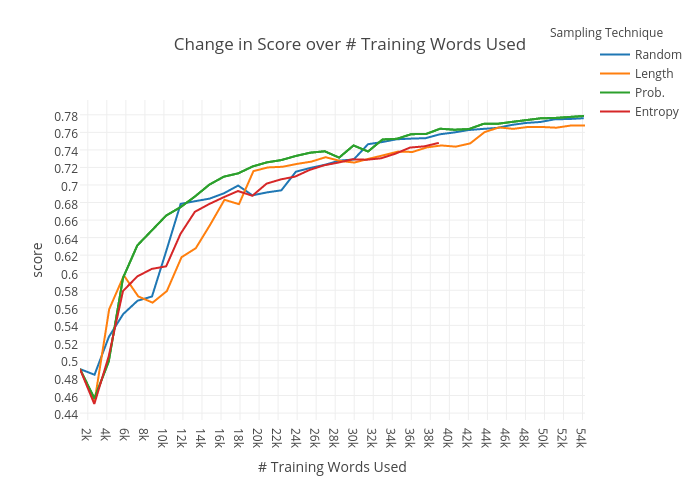
\includegraphics[width=115mm]{Change_in_Score_over___Training_Words_Usedcopy1.png}%
            \label{fig:right}%
        }
    \caption{\textit{Scores for the four selection techniques over number of words used.}}
    \label{fig:default}
\end{figure}

As mentioned in the introduction, given that the purpose here is to evaluate the selection techniques in the perspective of Active Learning, the below observations are mainly concerned with the early values for number of words used.

From the graph in Figure 1, the most surprising of all of the results is that entropy isn't necessarily the clear best despite being the main focus of Hwa's paper and intuitively being the the concept of disorder. Of the four selection techniques, the entropy-based selection is tied for being the second best. At no point, does entropy really overtake the probability in at the lower amount of words. 

On the other hand, the probabilistic selection method clearly does the best. It achieves an initial boost, having a score that is clearly larger than that of the baseline random, before beginning to converge the final probability. This is especially discernible at 6k to 12k words range in the graph.

Interestingly, length does better and worse than the baseline random at different parts in the initial segments of the curve. Specifically, the score initially looks like it shows a boost over random before fluctuating under the random curve before emerging ahead of random before convergence. In general, the length curve overall has some improvement for particular early regions of the curve in comparison to the baseline random curve, though not by much.

\subsection{Discussion}

The following subsections provide a discussion on the various patterns found in Figure 1. Note that the remainder of the discussion leverages entropy as mentioned in Hwa's paper. An improvement to the quantity is discussed in the Additional Experiments section (see Section 4.1).

\subsubsection{Awkward Initial Dip}

An interesting observation is that there is an initial dip in score performance for each of the  curves. The pattern is least pronounced in the random case while being quite pronounced in all of the others. No other segment of the curvature has this type of pattern.

Note that the initial training set included only the first fifty sentences found in the wsj/00 folder, while the additional training sentences used for active learning are from folders wsj/01, wsj/02, and wsj/03. One possible explanation for this phenomenon is that the model likely overfit to the initial training data and as the data from the additional training examples were provided, the model obtained a mixture that was temporarily worse than the initial case, due to the examples it actively selected based on the initial data alone. However, as more samples were added from the additional training data for active learning, all models began to perform better. This notion is reinforced by the fact that random selection, which doesn't really rely on the existing training data or the features of the additional training data, had the least pronounced dip. This also reinforces the notion that not all training data is equivalent.

\subsubsection{Where and Why Active Learning Helps}

The concept of Active Learning and the phenomenon discovered in the experiments can be explained through an analogy to students learning in a classroom from a professor. A professor can inundate a student with a great deal of information and explanations without any order or preference from the student. The student might slowly increment their overall knowledge from this. However, the student learns the fastest if he/she decides to clear up their existing doubts about the material by asking the professor for specific information regarding what they are uncertain about. In the analogy, the selection functions in active learning play the role of the decision the student makes about what they currently don't know or need to know further, the system being trained is the student, and the training mechanism with the annotated corpus of training examples is the professor.

Thus, in an ideal training scenario with an ideal selection function, Active Learning would always pick the most ideal example that would help the underlying classifier or system improve its learning the best. Active Learning, thus, only seeks to increment the speed at which a certain degree of competence is being approached not boost the eventual score. Note that all of the curves in Figure 1 converge to the same eventual score. Only the overall system implementation and the actual algorithm control the overall best possible score reached at the end. As with the student case, in time, all students might end up with the same amount of knowledge but the pace of learning the material might favor those who actively seek to clarify their doubts. As such, the benefit of Active Learning can be best be seen early on in the learning curves, where the better selection functions display better overall score performance. 

This is clear in the experiments, especially for the probability-based selection function. Note that actively learning based on the examples with the lowest best parse tree scores provided the maximum benefit. As in the analogy, removing the uncertainty about these parses helps the model leveraging the probability-based selection function reach higher scores early on. This further reinforces the notion that not all sets of training examples are equivalent. A particular set of training examples has the potential to stimulate significantly better training than a less than ideal set of training examples. In situations of resource constraint (e.g. time), Active Learning can be particularly useful in helping optimize the training being done for a given system.

\subsubsection{Comparing Selection Functions}

Note that not all selection functions are equal either. Continuing with the analogy, if the student selects to hear about concepts which are less useful in expanding their knowledge for a given situation, the overall knowledge gain rate for that material will suffer. This is apparent based on the curves in Figure 1, and as seen in Figure 1, the order of selection functions, with the best performance first, was:

\begin{enumerate}
\item Probability-based Selection
\item Entropy-based Selection
\item Length-based Selection
\item Random-based Selection
\end{enumerate}

In general, the advantages of the probability-based selection method over the length-based and random-based selection methods are immediately apparent. 

The normalized score of the best parse is an immediate indicator that the model performs poorly for that situation. Length, however, is not as direct in the assessment. Intuitively, sentence length has correlation with difficult sentences but it does not imply it as the score metric directly does. Therefore, there may be some situations where the length heuristic selects candidates which are ideal and situations where the length heuristic selects candidates that are less than ideal.

Similarly, randomized does little to select the best example to optimize training. Assuming a fair distribution of good examples in the training set, random selection has a chance of selecting some good examples. This helps explain why there are some boosts in performance. However, aside from small chance, it cannot best the probability-based selection, in general, in the case of Active Learning, because probability-based selection will consistently pick better training examples (again aside from chance).

The real surprise was tree entropy. Though the concept of entropy is ingrained with the notion of uncertainty and disorder, it performed worse than the probability baseline and just better than the other two. One potential explanation is irregularities within the data sets used. Another potential explanation is the normalizing term (i.e. sentence length) used by Hwa in the experiments. In the data utilized for the experiments in the assignment, a deeper inspection revealed that the normalizing term caused small sentences to be generally ordered to be selected first for learning. While longer length does not always imply the need to be selected first, there is somewhat of a correlation. The normalization might have worked for the selection of data Hwa attempted, but does not suit the data used in the experiments for this assignment. This idea is further explored in the Modifying the Entropy Selection Function section (see secton 4.2).

\subsubsection{Comparing Against Hwa's Results}

Overall, the experiments somewhat matched up with Hwa's results. Hwa utilized a random selection function for baseline, a sentence length based selection function, and the tree entropy based selection function. not all that good.

The results for length somewhat agree. In Hwa's results, the selection function leveraging the length heuristic performs quite close to the random baseline with a slight improvement, in both large set and small set cases. Though there are fluctuations, I, more or less, observe a similar, albeit fluctuating, improvement for length. The differences, again, could be due to the differences in regularity between the data sets used. Though Hwa also used WSJ as her source corpus, we still did not necessarily use the same data. In addition, the actual training parameters (e.g. the number of new sentences picked up, initial training data size, test data) are different. Therefore, I can expect that the results are somewhat different but show the same overall characteristics.

As mentioned in the previous section, the tree entropy results did not match at all. While Hwa saw a marked improvement by leveraging the selection function based on tree entropy, it was overshadowed by the probability-based selection in my experiments above. For the sake of brevity, I'm not repeating the my hypotheses for the presence of the stark difference, which was mentioned in the section above. 

\section{Additional Experiments}

The following subsections discuss the additional experiments that I ran.

\subsection{Varying Stopping Point For Iterations}

\subsubsection{Setup}

In order to empirically observe the behavior each of the curves at the limit, I changed the iteration stopping point value to 35. Given that the results from a 35 iteration run would encompass the results of all lower iteration value runs, I simply ran all the experiments for 35 iterations. 

\subsubsection{Experiment And Results}

Figure 2 captures the results from running each of the experiments for 35 iterations. 

\begin{figure}[h]%
	\centering
        \subfloat[]{%
        	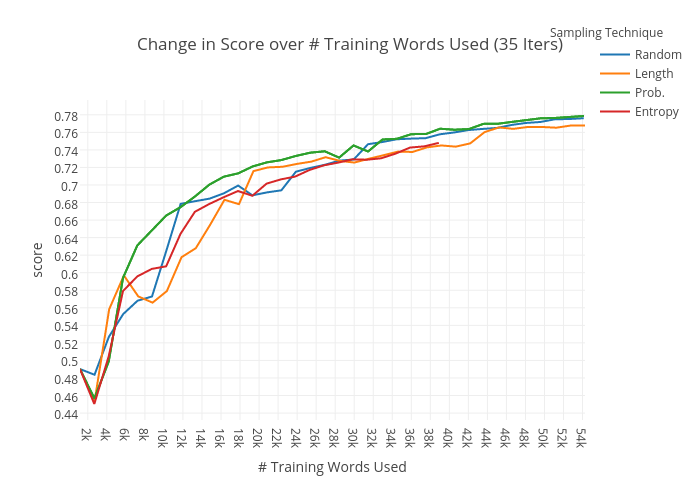
\includegraphics[width=115mm]{Change_in_Score_over___Training_Words_Used_iters.png}%
            \label{fig:right}%
        }
    \caption{\textit{Scores for the four selection techniques over number of words used.}}
    \label{fig:default}
\end{figure}

In general, increasing the iterations allows all of the curves to converge to a certain point. An extremely high iteration value run has no significant gain on the Active Learning since values will eventually converge at limit. Lower iteration runs, however, has a lot to benefit from Active Learning. Given that iterations correspond with words used for training, Figure 1 shows that at lower word counts, an Active Learning approach with a good selection function will provide much better performance than a vanilla approach or a poor selection function. This behavior can be attributed to the nature of Active Learning attempting to optimize the iterations/words necessary to reach a specific high score.


\subsection{Modifying the Entropy Selection Function}

\subsubsection{Setup}

Based on my hypothesis in section 3.4.3, I modified the entropy function to not normalize on sentence length. I, then, ran the experiment for entropy with the same parameters as before.

\subsubsection{Experiment and Results}

Figure 3 shows the modified selection function with the other functions.

\begin{figure}[h]%
	\centering
        \subfloat[]{%
        	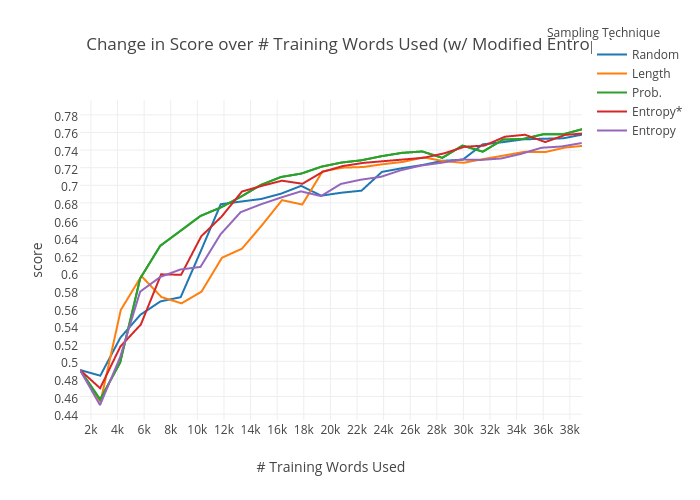
\includegraphics[width=115mm]{Change_in_Score_over___Training_Words_Used_entropy.png}%
            \label{fig:right}%
        }
    \caption{\textit{Updated scores with the modified entropy function used (Updated entropy function labeled as Entropy*).}}
    \label{fig:default}
\end{figure}

By not normalizing on the sentence length, there was a small boost in performance. In particular, the entropy-based selection function was clearly the second best with the modification. However, the selection function based on the probability of the best parse still clearly was the top choice, despite the modification. This is mainly discernible in the range between 4k and 14k words. Beyond that range, Entropy* does just as well but the fact that the probability score based function has a clear advantage is some of the earlier pieces of the curve places it in better position in the context of Active Learning. In addition, this suggests that the removal of the normalization step may not be exactly or only what needs to be modified in order to use the metric accounting for a larger range of data irregularities.

\subsection{Varying K For Entropy}

\subsubsection{Setup}

To test the difference the tree entropy strategy makes at different K, I tested three other values for K (e.g. the constant indicating the number of top parses to use in the entropy computation): 5, 15, 20. All other values remained the same as with the experiments described in Selection Methods Experiments section (i.e. the required experiments). 

\subsubsection{Experiment and Results}

Figure 4 shows the results of varying the K parameter.

\begin{figure}[h]%
	\centering
        \subfloat[]{%
        	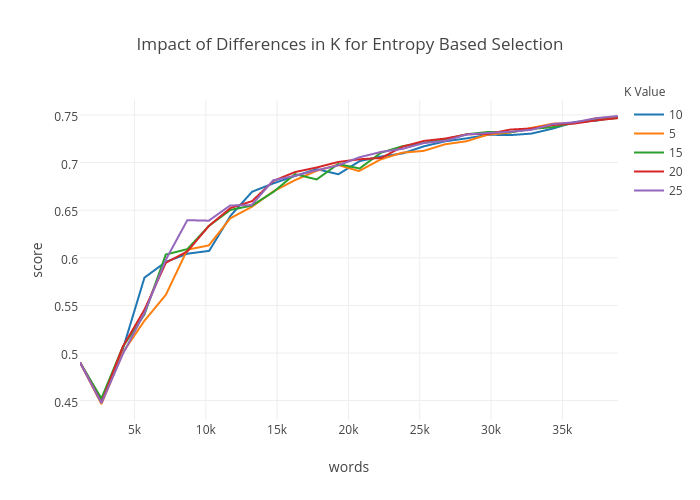
\includegraphics[width=115mm]{Impact_of_Differences_in_K_for_Entropy_Based_Selection}%
            \label{fig:right}%
        }
    \caption{\textit{Updated scores with the modified entropy function used (Updated entropy function labeled as Entropy*).}}
    \label{fig:default}
\end{figure}

Overall, the results were not significantly distinct from one another for the various values of K as seen in Figure 4. The results are close enough to really not have a clear winner. This points out the possibility that selecting a set of top K parses provides most of the necessary information for the computation of the entropy. Adding further information beyond a K may not provide a significant extra boost. This observation might be especially important in a real-world situation where performance is key. A larger set of top parses to compute entropy might involve higher costs in performance. As a result, it might be best to simply select an optimal top K values if the overall gain begins to taper after a certain point. 

\subsection{Varying Training Batch Size}

\subsubsection{Setup}

To test the impact of variation in batch size (e.g. the amount of words to be taken per round), I tested against two other batch values: 1000 and 2000. All other values remained the same as with the experiments described in the Selection Methods Experiments section.

\subsubsection{Experiment and Results}

Figure 5 shows the results of varying the batch size.

\begin{figure}[h]%
	\centering
        \subfloat[Random]{%
        	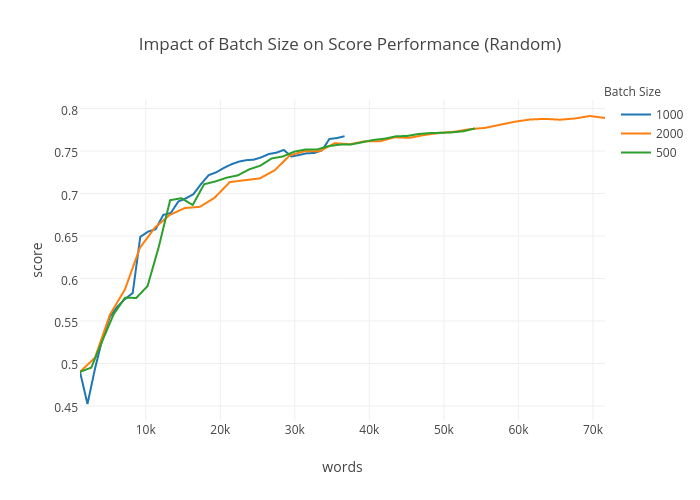
\includegraphics[width=80mm]{Impact_of_Batch_Size_on_Score_Performance__Random_.png}%
            \label{fig:right}%
        }\hfill%
        \subfloat[Length]{%
        	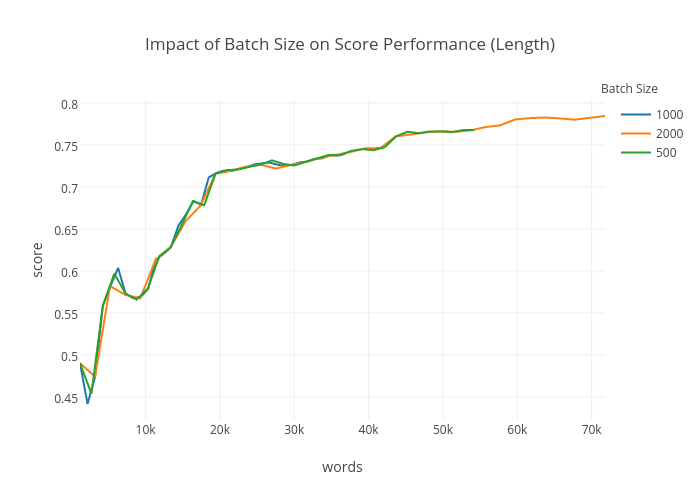
\includegraphics[width=80mm]{Impact_of_Batch_Size_on_Score_Performance__Length_.png}%
            \label{fig:right}%
        }\hfill%
        \subfloat[Probability]{%
        	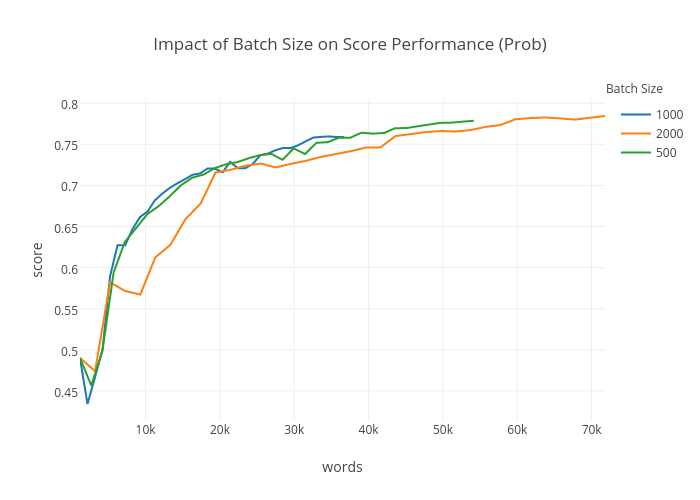
\includegraphics[width=80mm]{Impact_of_Batch_Size_on_Score_Performance__Prob_.png}%
            \label{fig:right}%
        }\hfill%
        \subfloat[Entropy]{%
        	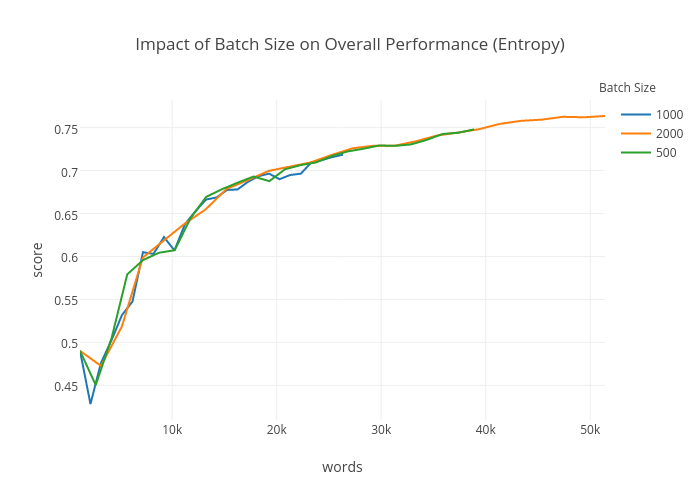
\includegraphics[width=80mm]{Impact_of_Batch_Size_on_Overall_Performance__Entropy_.png}%
            \label{fig:right}%
        }
    \caption{\textit{Impact of changing the batch size of examples selected each round on the four different selection functions.}}
    \label{fig:default}
\end{figure}

Based on Figure 5, variation in the selection of batch size has the biggest impact on selection orders that have changes of significant after every round (e.g. Probability). For those who are always constant order (e.g. Length), batch is really just equivalent to running more iterations. This is clear on the length selection function's curves in Figure 5b. For the ones who change order after each round, such as probability, the selection of batch size becomes extremely important. Too large of a batch size as seen with Figure 5c in the 2000 case suboptimally trains on too many examples. If the number of training examples can be thought of as a cost, it could optimally train on a smaller set of examples and use the increased knowledge from that shorter training to better select the remainder training examples. The failure to do this is why the 2000 case in Figure 5c performs worse initially than the others. Too small of a batch size, on the other hand, implies inefficiency, as there is constant ordering of the remainder of the training examples, which could be potentially large. Therefore, the selection of the batch size is an important task that needs to create balance based on the above concerns.

\subsection{Varying Initial Training Set Size}

\subsubsection{Setup}

To test the impact of variation in the initial training set size (e.g. the amount of words to be taken per round), I tested against three other initial training set values: taking in the first 100, 150, and 200 sentences respectively. All other experiment parameter values remained the same as with the experiments described in the Selection Methods Experiments section.

\subsubsection{Experiment and Results}

Figure 6 displays the impact of modifying the initial training set size across the different selection functions. 


\begin{figure}[h]%
	\centering
        \subfloat[Random]{%
        	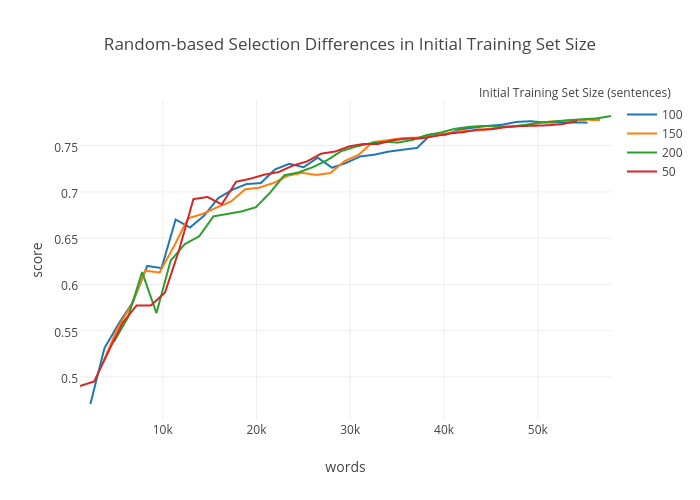
\includegraphics[width=80mm]{Random-based_Selection_Differences_in_Initial_Training_Set_Size.png}%
            \label{fig:right}%
        }\hfill%
        \subfloat[Length]{%
        	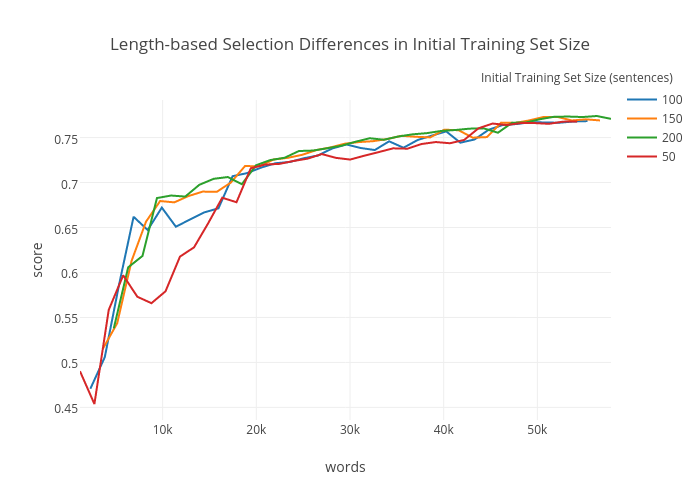
\includegraphics[width=80mm]{Length-based_Selection_Differences_in_Initial_Training_Set_Size.png}%
            \label{fig:right}%
        }\hfill%
        \subfloat[Probability]{%
        	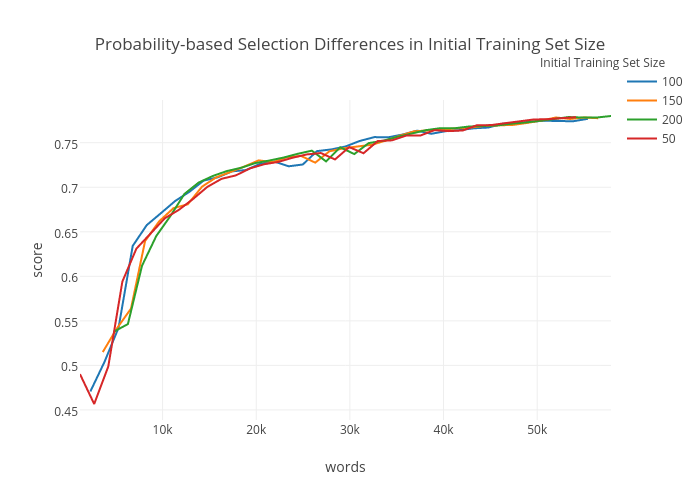
\includegraphics[width=80mm]{Probability-based_Selection_Differences_in_Initial_Training_Set_Size.png}%
            \label{fig:right}%
        }\hfill%
        \subfloat[Entropy]{%
        	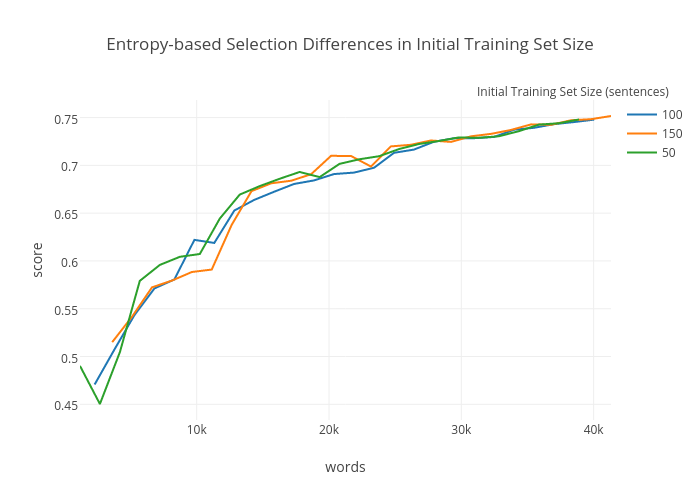
\includegraphics[width=80mm]{Entropy-based_Selection_Differences_in_Initial_Training_Set_Size.png}%
            \label{fig:right}%
        }
    \caption{\textit{Impact of changing the size of the initial training set on the four different selection functions.}}
    \label{fig:default}
\end{figure}

Based on Figure 6, the change in initial training set size has a small improvement in the overall performance for Active Learning. Given that we're concerned only with the shape at the beginning of the curvature for Active Learning, of the curves in Figure 6, only the Length curve displayed any sort of impact from the change in training size. In particular, the dip in score for the 50 case is removed. This is likely because the additional training examples helps bootstrap the overall system model better initially by giving it a larger range of examples. Recall the earlier point that length correlates with difficulty in a sentence but does not imply it. Therefore, the addition of the samples through this selection function does not necessarily need to pick the most helpful examples at each point. Essentially, the missing information from failure to pick the most helpful example is somewhat covered by the extra initial examples. This likely prevents the dip from the 50 case. We can note that the Probability and the Entropy cases select from their worst current parses so they avoid this problem entirely and don't display the same improvement in behavior as length.

\end{document}